\begin{equation}
    \begin{gathered}
        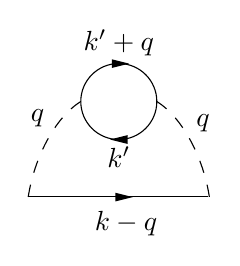
\begin{tikzpicture}[x=0.75pt,y=0.75pt,yscale=-0.7,xscale=0.7]
            %uncomment if require: \path (0,300); %set diagram left start at 0, and has height of 300
            
            %Straight Lines [id:da3041484358604427] 
            \draw    (76,155) -- (199.71,155) ;
            %Straight Lines [id:da07378190318685784] 
            \draw    (148,155.12) ;
            \draw [shift={(148,155.12)}, rotate = 180] [fill={rgb, 255:red, 0; green, 0; blue, 0 }  ][line width=0.08]  [draw opacity=0] (12,-3) -- (0,0) -- (12,3) -- cycle    ;
            %Shape: Circle [id:dp47981680317475917] 
            \draw   (112.17,89.33) .. controls (112.17,74.88) and (123.88,63.17) .. (138.33,63.17) .. controls (152.78,63.17) and (164.5,74.88) .. (164.5,89.33) .. controls (164.5,103.78) and (152.78,115.5) .. (138.33,115.5) .. controls (123.88,115.5) and (112.17,103.78) .. (112.17,89.33) -- cycle ;
            %Straight Lines [id:da9057585470587182] 
            \draw    (145.5,63.25) ;
            \draw [shift={(145.5,63.25)}, rotate = 180] [fill={rgb, 255:red, 0; green, 0; blue, 0 }  ][line width=0.08]  [draw opacity=0] (12,-3) -- (0,0) -- (12,3) -- cycle    ;
            %Straight Lines [id:da6868030069609872] 
            \draw    (138.33,115.5) -- (134.33,115.5) ;
            \draw [shift={(132.33,115.5)}, rotate = 360] [fill={rgb, 255:red, 0; green, 0; blue, 0 }  ][line width=0.08]  [draw opacity=0] (12,-3) -- (0,0) -- (12,3) -- cycle    ;
            %Curve Lines [id:da7139348254177498] 
            \draw  [dash pattern={on 4.5pt off 4.5pt}]  (76,155) .. controls (80,128.67) and (94,100.67) .. (112.17,89.33) ;
            %Curve Lines [id:da945710836678433] 
            \draw  [dash pattern={on 4.5pt off 4.5pt}]  (200.67,155) .. controls (196.67,128.67) and (182.67,100.67) .. (164.5,89.33) ;
            
            % Text Node
            \draw (120,163.08) node [anchor=north west][inner sep=0.75pt]    {$k-q$};
            % Text Node
            \draw (138.33,118.9) node [anchor=north] [inner sep=0.75pt]    {$k'$};
            % Text Node
            \draw (138.33,59.77) node [anchor=south] [inner sep=0.75pt]    {$k'+q$};
            % Text Node
            \draw (76,93.4) node [anchor=north west][inner sep=0.75pt]    {$q$};
            % Text Node
            \draw (190,96.4) node [anchor=north west][inner sep=0.75pt]    {$q$};
            \end{tikzpicture}            
    \end{gathered} \sim e^4 \int \dd[3]{\vb*{q}} \frac{1}{q^2} \frac{1}{q^2} \sim e^4 \frac{1}{q},
    \label{eq:most-divergent-1}
\end{equation}